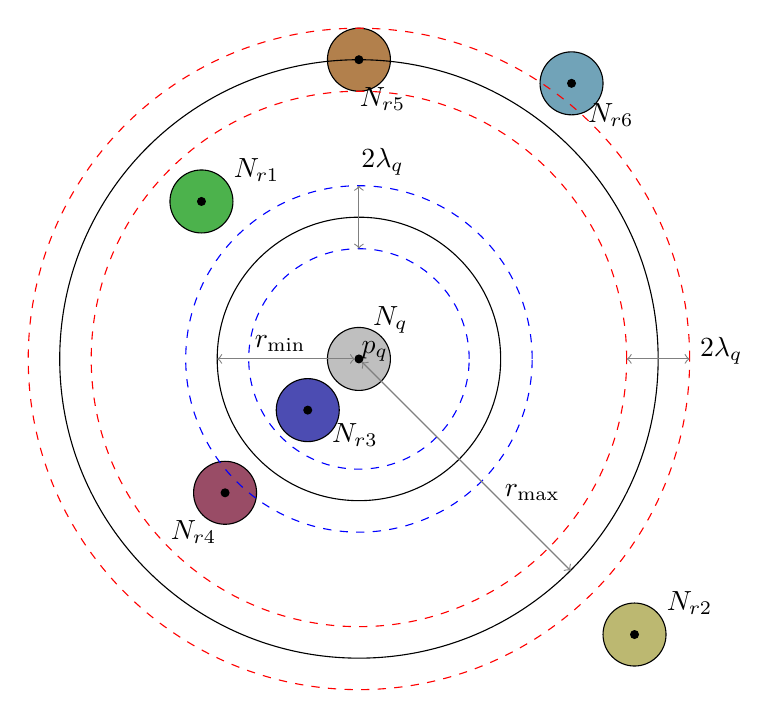
\begin{tikzpicture}
  % N_q
  \draw [fill=lightgray] (0, 0) circle (0.4);
  \node [ ] at (0.4, 0.5) { $\mathscr{N}_q$ };

  % p_q
  \node [draw, circle, inner sep=1pt, fill] at (0, 0) { };
  \node [ ] at (0.2, 0.1) { $p_q$ };

  % N_{r1}
  \draw [fill=green!40!gray] (-2.0, 2.0) circle (0.4);
  \node [draw, circle, inner sep=1pt, fill] at (-2.0, 2.0) { };
  \node [ ] at (-1.3, 2.4) { $\mathscr{N}_{r1}$ };

  % N_{r2}
  \draw [fill=yellow!40!gray] (3.5, -3.5) circle (0.4);
  \node [draw, circle, inner sep=1pt, fill] at (3.5, -3.5) { };
  \node [ ] at (4.2, -3.1) { $\mathscr{N}_{r2}$ };

  % N_{r3}
  \draw [fill=blue!40!gray] (-0.65, -0.65) circle (0.4);
  \node [draw, circle, inner sep=1pt, fill] at (-0.65, -0.65) { };
  \node [ ] at (-0.05, -0.97) { $\mathscr{N}_{r3}$ };

  % N_{r4}
  \draw [fill=purple!40!gray] (-1.7, -1.7) circle (0.4);
  \node [draw, circle, inner sep=1pt, fill] at (-1.7, -1.7) { };
  \node [ ] at (-2.1, -2.2) { $\mathscr{N}_{r4}$ };

  % N_{r5}
  \draw [fill=orange!40!gray] (0, 3.8) circle (0.4);
  \node [draw, circle, inner sep=1pt, fill] at (0, 3.8) { };
  \node [ ] at (0.3, 3.3) { $\mathscr{N}_{r5}$ };

  % N_{r6}
  \draw [fill=cyan!40!gray] (2.7, 3.5) circle (0.4);
  \node [draw, circle, inner sep=1pt, fill] at (2.7, 3.5) { };
  \node [ ] at (3.2, 3.1) { $\mathscr{N}_{r6}$ };

  % l
  \draw (0, 0) circle (1.8);
  % l - \lambda_q
  \draw [blue, dashed] (0, 0) circle (1.4);
  % l + \lambda_q
  \draw [blue, dashed] (0, 0) circle (2.2);

  % u
  \draw (0, 0) circle (3.8);
  % u - \lambda_q - \lambda_r
  \draw [red, dashed] (0, 0) circle (3.4);
  % u + \lambda_q + \lambda_r
  \draw [red, dashed] (0, 0) circle (4.2);

  % line from p_q to l
  \draw [gray, arrows=<->] (-0.05, 0) -- (-1.8, 0);
  \node [ ] at (-1.0, 0.2) { $r_{\min}$ };

  % line from p_q to u
  \draw [gray, arrows=<->] (0.04, -0.04) -- (2.687, -2.687);
  \node [ ] at (2.2, -1.7) { $r_{\max}$ };

  % line indicating u shell
  \draw [gray, arrows=<->] (4.2, 0) -- (3.4, 0);
  \node [ ] at (4.6, 0.1) { $2\lambda_q$ };

  % line indicating l shell
  \draw [gray, arrows=<->] (0, 2.2) -- (0, 1.4);
  \node [ ] at (0.3, 2.5) { $2 \lambda_q$ };

\end{tikzpicture}
